%Gloss
%\input{if-glossary} % this isn't working 4/13/14

%Abst
%\input{workbook1/if-wkbk-abstract}  Worry about this later... (AH)

\chapter{How to Read this Documentation}
\label{ch:how-to-read}

This is the introduction

\section{If you are new to HEP Software...}

Section 1 of chapter 1


\section{If you are an HEP Software expert...}

Section 2 of chapter 1

\chapter{The Next Chapter}
\label{ch:next_chapter}

This is chapter 2 and refers to Figure~\ref{fig:interfaceTDAQ}

\begin{figure}[tbp]
\centering
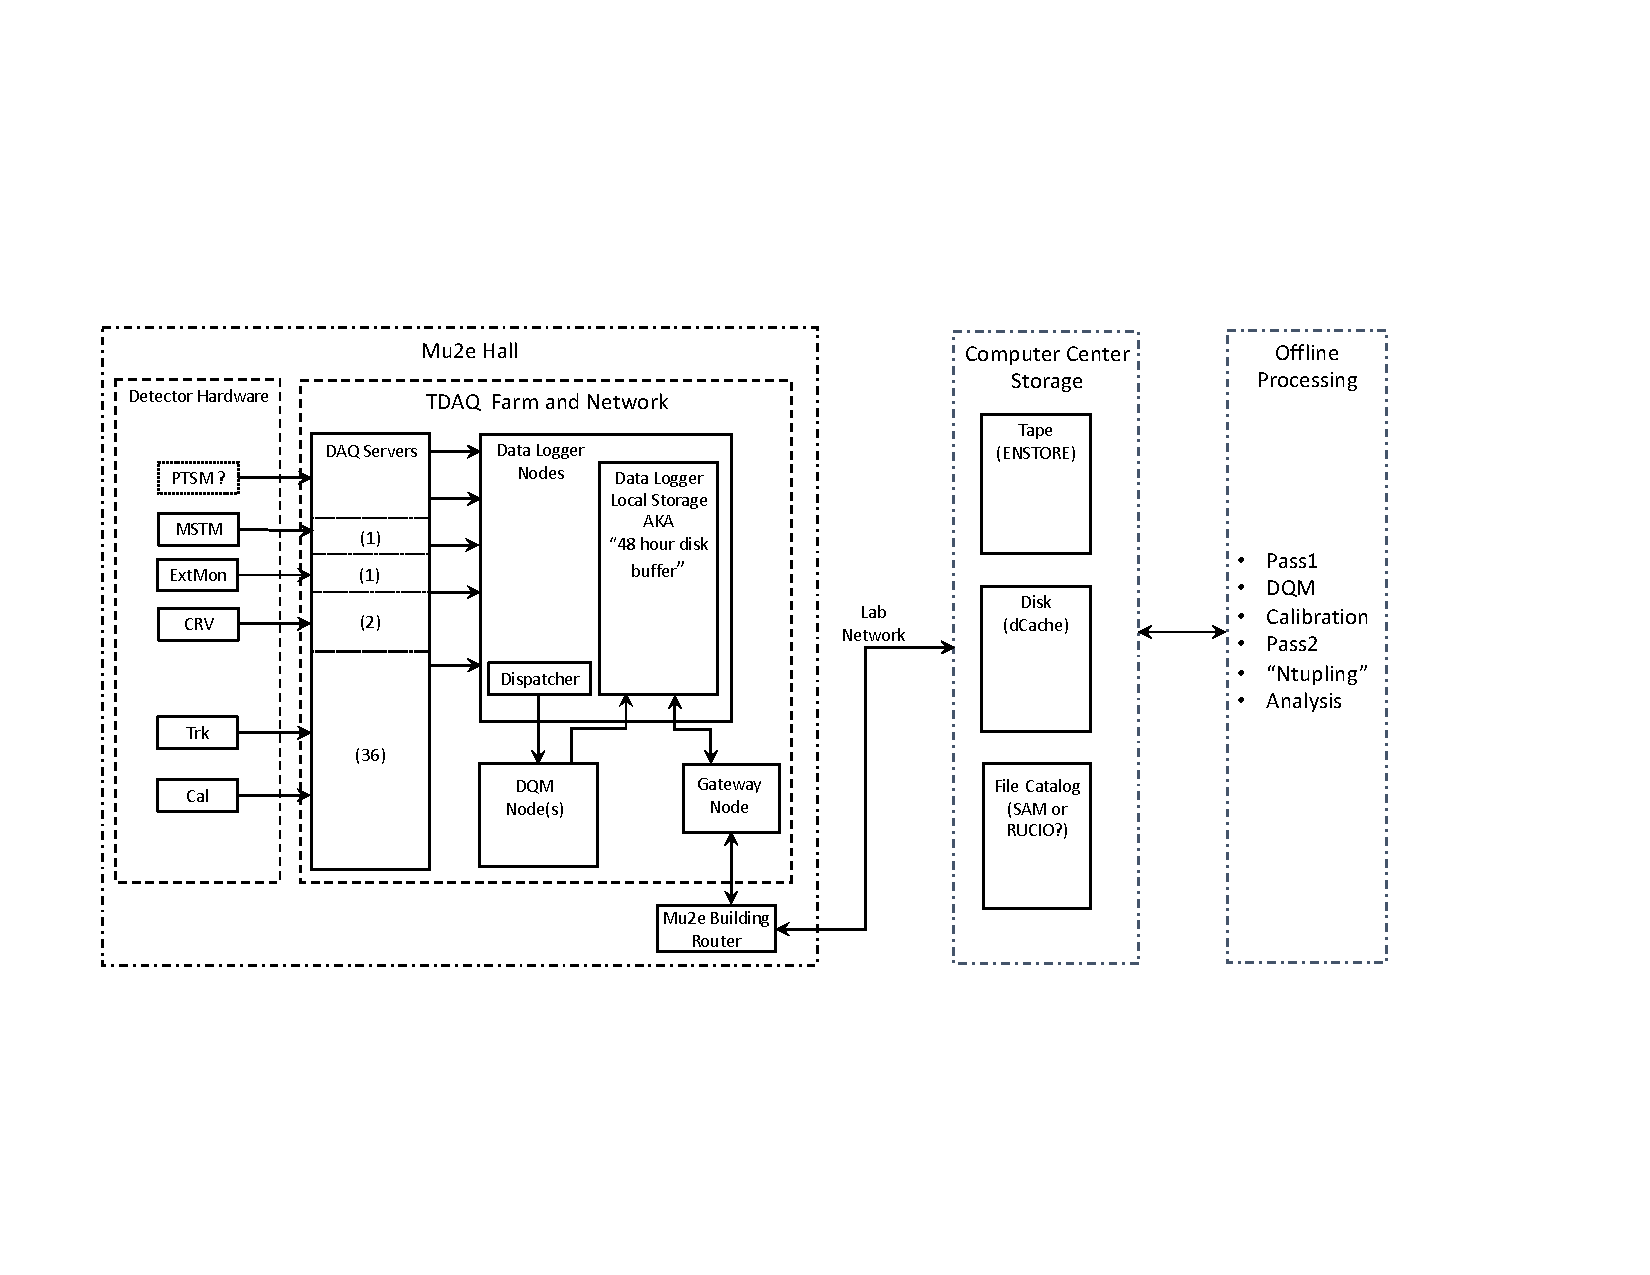
\includegraphics[width=0.9\textwidth]{figures/interface_with_TDAQ.pdf}
\caption{The interface with the TDAQ System}
\label{fig:interfaceTDAQ}
\end{figure}


\section{If you are new to HEP Software...}

Section 1 of chapter 2


\section{If you are an HEP Software expert...}

Section 2 of chapter 2


% Keep sections under development
\IfStrEq{\ISDRAFT}{YES}{

\chapter{A Chapter under development}
\label{ch:under_development}

This is a chapter still under development

\section{If you are new to HEP Software...}

Section 1 of a chapter still under development


\section{If you are an HEP Software expert...}

Section 2 of a chapter still under development

} % end `ISDRAFT = YES'


\appendix

\chapter{SubRuns}
\label{ch:app_Subruns}

This appendix has information about subruns

\section{If you are new to HEP Software...}

Section 1 of the appendix on subruns that refers to Table~\ref{tab:clhep:functions}.
\begin{table}
\begin{center}
\caption[Selected member functions of {\tt CLHEP::Hep3Vector}]{Selected member functions of {\tt CLHEP::Hep3Vector}.}
\label{tab:clhep:functions}
\begin{tabular}{lll}\hline
  {\cppfcl a = u.cosTheta();}  & {\cppfcl double cosTheta() const;} & $\cos\theta$\\
  {\cppfcl a = u.cos2Theta();} & {\cppfcl double cos2Theta() const;} & $\cos^2\theta$\\
  {\cppfcl v = u.unit();}      & {\cppfcl Hep3Vector unit() const;} & A unit vector in the direction of {\cppfcl u} \\ \hline
  \end{tabular}
\end{center}
\end{table}


\section{If you are an HEP Software expert...}

Section 2 of the appendix on subruns.

\chapter{DQM Data}
\label{ch:DQM data}

This appendix has information about subruns

\section{If you are new to HEP Software...}

Section 1 of the appendix on subruns.


\section{If you are an HEP Software expert...}

Section 2 of the appendix on subruns.

\cleardoublepage
\printindex

